\chapter{Design}\label{chapter:design}

\section{The Algorithm: An Abstract Description}\label{sec:abstract_algo}

\subsection{Definitions}\label{sec:definitions}

Emulators, or binary translators in general, take as input machine instructions of an \ac{ISA} $X$ and produce
semantically equivalent instructions for an \ac{ISA} $Y$. In the special case of emulators, we call $X$ the
\textit{guest} \ac{ISA} and $Y$ the \textit{host} \ac{ISA}.

% Definition 'Program'
A program $P_X = (x_i)_{1 \leq i \leq n}$ of an \ac{ISA} $X$ is a series of $n$ instructions, each of which is a mapping
of program states $S_i \mapsto x_i(S_i)$. Thus, a program can be expressed as
    $P_X : S_1 \mapsto S_{n+1} = x_n(S_n)$
with an arbitrary fixed input state $S_1$. Two programs are \textbf{semantically equivalent} if $P_X(S) = P_Y(S)$ for
all input states $S$. In this case, we write $P_X \equiv P_Y$.

% Definition 'translator', local discreteness
A binary translator (which may be an emulator) can be modelled as a function $E_{X \rightarrow Y}: P_X \mapsto P_Y$. It
is \textbf{correct} if the output program is semantically equivalent to the input program:
    $P_X \equiv E_{X \rightarrow Y}(P_X)$.
A binary translator is \textbf{locally discrete}, or context-independent, if it achieves $P_X \mapsto P_Y$ by mapping
each guest instruction individually to a semantically equivalent host program:
\begin{equation}\label{eq:locally_discrete}
    E_{X\rightarrow Y}(P_X) = E_{X \rightarrow Y}((x_i)_{1 \leq i \leq n}) = (E_{X \rightarrow Y}(x_i))_{1 \leq i \leq n} = P_Y
\end{equation}
with $E_{X\rightarrow Y}(x_i) \in \mathcal{P}_Y$ (where $\mathcal{P}_Y$ is the set of all programs of $Y$). In other
words, $E_{X\rightarrow Y}$ is distributive with respect to function application in $X$. Note that single instructions
are programs by the definition above ($\forall x \in X: x \in \mathcal{P}_X $), meaning the argument to an emulator
function $E$ can be a single instruction or a series of instructions, i.e., a program.

% Result local equivalence => global equivalence
If the semantic equivalence condition holds for each translation unit individually, it follows that it also holds globally:
\begin{equation}\label{eq:local_to_global_discreteness}
    x_i \equiv E_{X\rightarrow Y}(x_i) \forall i \implies (x_i) \equiv (E_{X\rightarrow Y}(x_i)) \implies P_X \equiv P_Y
\end{equation}

\subsection{Testing Program Equivalence}\label{sec:program_equiv}

Focaccia tests the correctness of emulators (refer to section~\ref{sec:testing}): formally, it takes on the endeavour of
implementing the equivalence check $P_X \equiv E_{X \rightarrow Y}(P_X)$. To make this problem tractable (because a
non-simplified version is essentially the concern of formal verification methods, which are rarely realistically
applicable to large programs, and certainly not in an automated way), we can exploit the fact that binary translators
are always implemented as locally discrete translators and combine that with the result from
equation~\ref{eq:local_to_global_discreteness}: We now check whether $x_i \equiv E_{X \rightarrow Y}(x_i)$ for all $x_i
\in P_X$, which implies $P_X \equiv E_{X \rightarrow Y}(P_X)$.

Attempts to solve this equivalence directly bear the following problems:

\begin{enumerate}
    \item We need to find $x$. Usually, an \ac{ISA} does not have a canonical way to represent its instructions as
        manipulable functions.
    \item We need to find $E_{X \rightarrow Y}(x)$.
    \item We need to determine when $x \equiv y$.
    \item Comparing $x \equiv y$ is not enough, even if it were feasible, because the translation $E_{X \rightarrow
        Y}(x) = (y_j)_{1 \leq j \leq m} \in \mathcal{P}_Y$ may be a series of \textbf{multiple} instructions in $Y$, so
        the true question expands to: When is $x \equiv (y_j)$?
\end{enumerate}

Theorem solvers that can tackle problems 3 and 4 exist; an example is Microsoft's Z3 theorem
prover~\cite{Z3prover2024Mar}. Problem 2, however, makes this direct approach impossible. To elaborate: Static binary
translators output the translation as generated machine code, but dynamic binary translators, on which our focus lies,
do not. Emulators implement guest instructions opaquely in complex high-level language code and cannot extract the
abstract equation that is implemented by this code, meaning it cannot know or communicate $E(x)$---the impossibility of
solving problem 2 directly is the premise on which Focaccia is useful.

To circumvent this unsolvable requirement, we can restate the problem and test whether $x(S) = [E_{X \rightarrow
Y}(x)](S)$, which by definition implies $x \equiv E_{X \rightarrow Y}(x)$. This means that we have to find the
emulator's \textbf{state} rather than its action on states. The set of problems to solve reduces to:

\begin{enumerate}
    \item We need to find $S = x(S_0)$. We call $S$ the \textit{truth state}: it is the state that results when an
        instruction $x$ is correctly applied to an initial program state $S_0$.
    \item We need to find $S^E = [E_{X \rightarrow Y}(x)](S_0)$. We call $S^E$ the \textit{test state}; it is obtained
        by executing the translation of $x$ on an initial program state $S_0$. Section~\ref{sec:obtaining_snapshots} is
        concerned with this task.
    \item We need to determine when $S = S^E$. As program states $S$ are constants, their equality is theoretically
        trivial. Practically, however, the respective initial states of the native program and the translated program
        are often not precisely equal. Therefore we implement an equivalence operator $S \equiv S^E$ which represents an
        equality with respect to differing start states. Section~\ref{sec:comparison} explores this necessity in detail.
\end{enumerate}

\subsection{Local Discreteness}\label{sec:local_discreteness}

It was argued that requiring a tested translator to satisfy local discreteness is imperative to verifying whether $P_X
\equiv P_Y$ when dealing directly on the level of equivalences; $\mathcal{P}_X$ and $\mathcal{P}_Y$ are infinitely
large, therefore a divide-and-conquer approach is inevitably necessary.

However, when we use the definition of semantical program equivalence to transform the problem from $P_X \equiv E_{X
\rightarrow Y}(P_X)$ to $P_X(S) = [E_{X \rightarrow Y}(P_X)](S)$, the global comparison of result states becomes
possible again.  While this removes the theoretical necessity for the local discreteness assumption, it is still
practically useful, if not essential. An outcome of comparing result states of full program executions would be a
statement like "The program's translation is erroneous". This is too general of an assertion to be useful to
developers. When we instead use local discreteness and check for all intermediate states whether $S_i = S^E_i$ (where
$S_i = x_{i-1}(S_{i-1})$ and $S^E_i = E_{X \rightarrow Y}(x_{i-1})(S^E_{i-1})$, with $S_1 = S^E_1$ an arbitrary initial
state), we can generate much more detailed information, such as "Instruction $x_i$ is translated incorrectly because
$S_i \neq S^E_i$~". This is exactly the type of feedback that Focaccia seeks to provide.

Additionally, it lets the algorithm recover from errors: Even if an instruction $x_i$ turns out to be implemented
incorrectly, thus producing an incorrect state $S^E_{i+1}$, that state is only incorrect from the viewpoint of program
semantics. The verifier, however, can still treat it as a valid input state to all subsequent instructions $x_{j > i}$
because the translation $E_{X \rightarrow Y}(x_j)$ is required to be \textit{locally correct} for a locally discrete
translator, that is, it must work correctly on \textbf{any} program state.

Note that it is valid to assume an emulator's implementation to be locally discrete because it is not only by far the
most feasible strategy to implement any binary translator, but also the core axiom of dynamic binary translation itself:
an emulator is \textbf{defined} as an online interpreter that operates with only a local view on the program.

A first version of a verification algorithm could thus look as follows: We run $P_X$ on one initial state $S_1$ and the
translation $E_{X \rightarrow Y}(P_X)$ on the same initial state, during which we record intermediate states of each
execution, obtaining two respective lists of program states $(S_1, S_2 = x_1(S_1), S_3 = x_2(S_2), …)$ and $(S^E_1,
S^E_2 = E_{X \rightarrow Y}(x_1)(S_1), S^E_3 = E_{X \rightarrow Y}(x_2)(S^E_2), …)$ with $S_1 = S^E_1$. For each pair of
states $(S_i, S^E_i)$, we test whether $S_i = S^E_i$. If this equality does \textbf{not} hold, then $x_i \not\equiv E_{X
\rightarrow Y}(x_i)$, meaning the translator's implementation of $x_i$ is faulty.

\subsection{Comparing Program States}\label{sec:comparison}

The algorithm requires an equality operator on program states: $S = S'$. An intuitive way of implementing this operator
is by comparing the register- and memory content. These values are what constitute the state of a program, and they are
numeric values with a canonical condition for equality. However, as section~\ref{sec:program_equiv} indicated, comparing
program states is more complex in reality. That is because the starting states for the execution of programs are not
always equal: the previous assumption that $S_1 = S^E_1$ is not necessarily true. In fact, it is most commonly false.
Possible contributing factors (subsequently collectivized as a general \textit{difference in environment}) include:

\begin{itemize}
    \item Different initial stack pointers.
    \item Different addresses of heap allocations.
    \item Different environment- and auxiliary vectors. The latter is particularly interesting. It turns out that
        the auxiliary vector provided by QEMU, for example, routinely differs from the one provided by the operating
        system. See section~\ref{sec:auxv} for more details.
\end{itemize}

Therefore, instead of comparing $P_X(S) = P_Y(S')$, which does \textbf{not} imply $P_X \equiv P_Y$ if $S \neq S'$, the
comparison must take into account the initial difference $\Delta_S = S - S'$ and establish a \textbf{state equivalence}
$P_X(S) \equiv_{\Delta_S} P_Y(S') \implies P_X \equiv P_Y$ with respect to it.
%This is the chief nontriviality that Focaccia's algorithm solves.

The way we calculate this equivalence is by re-introducing information about the guest instructions $x_i$ to the
algorithm which, in order to simplify the problem, we have discarded when we transformed the central question from $x
\equiv E_{X \rightarrow Y}(x)$ to $x(S) = [E_{X \rightarrow Y}(x)](S)$. The new algorithm works as follows: Instead of
running guest program and translation in parallel and comparing their intermediate states, only run the translation
$E_{X \rightarrow Y}(P_X)$ on a start state $S^E_1$, thereby obtaining the translation's intermediate states $S^E_i$.
Then, for each $S^E_i$, use the guest instruction $x_i$ to calculate a corresponding \textbf{expected state} $S_{i+1} =
x_i(S^E_i)$. These represent truth states that would result from executing $x_i$ on $S^E_i$ if $x_i$ was implemented
correctly. Finally, compare the expected state to the actual translation state: $S^E_{i+1} = S_{i+1}$. Again, this works
because it does not matter to the verifier whether $S^E_{i+1}$ is a \textit{correct} state with regards to whole-program
semantics.

Decomposing the pre-translation program $(x_i)$ into its instructions and applying them selectively to the synthetic
test states as opposed to executing it natively on a semi-random starting state thus allows us to use the same starting
state for both the translation and the truth program at each instruction, eliminating $\Delta_S$. This enables the
desired equality comparison $x_i(S_i) = E_{X \rightarrow Y}(x_i)(S_i)$. The drawback of this approach is that we now
require an additional piece of information: We need to know $x_i$.

Not only do we need to know what every $x_i$ is, but we also demand a way of applying it individually to an arbitrary
program state we determine or, more precisely, which is being determined by the translation's execution. One approach
would be to generate and run a small program or piece of code that sets up the correct machine state, then runs the
instruction in question, and finally reads the resulting state back. We chose a different path: We use symbolic
execution tools to translate instructions into equations, which we manually apply to the states we want to test.
Section~\ref{sec:symb_exec} explains how this works.

% Explanation of the comparison algorithm from Overview, from which I had to remove all math:
%
%The primary emulator verification algorithm requires as inputs:
%
%\begin{itemize}
%    \item A concrete test trace $((x_1, S_1), …, (x_n, S_n))$. This is a trace of the program $P_X = (x_i)$'s execution
%        via the tested emulator. It comprises program state snapshots $S_i$ (which contain the process's concrete
%        register- and memory contents before $x_i$ is executed) for each emulated instruction $x_i$.
%    \item A symbolic reference trace $(\sigma_1, …, \sigma_n)$. This is the oracle. It is a trace of the same program,
%        but, instead of program snapshots, it defines symbolic equations that encapsulate the corresponding
%        instruction's \textit{correct} behaviour: $\sigma_i(S) = x_i(S)$ for any program state $S$.
%\end{itemize}
%
%For each instruction and program snapshot $(x_i, S_i)$ in the concrete trace, the verifier uses the corresponding
%symbolic equation $\sigma_i$ to predict the next concrete state $S'_{i+1} = \sigma_i(S_i) = x_i(S_i)$, which is the
%expected outcome if instruction $x_i$ acted on $S_i$ correctly. It then tests whether $S'_{i+1} = S_{i+1}$ (where
%$S_{i+1} = E(x_i)(S_i)$, $E$ the tested emulator), meaning it compares whether the emulator's state matches the expected
%state. Another way to think about this is that the verifier calculates a state difference $\Delta_{S_{i+1}} = S'_{i+1}
%- S_{i+1}$. If $\Delta_{S_{i+1}} \neq 0$, then the emulator's state diverges from the truth state, meaning its
%translation of $x_i$ is faulty and a detailed error message is generated that includes the faulty instruction, the
%expected transformation $\sigma_i$, and the changes in values that the emulator has actually (wrongly) calculated.

\section{Symbolic Execution}\label{sec:symb_exec}

The task at hand is to find a representation of any instruction $x$ that encapsulates the semantics of the
transformation it applies to program states on which it is executed and is able to calculate that operation on synthetic
program states. Focaccia uses symbolic execution tools to translate instructions into symbolic equations that do
precisely that. It turns out that if one executes an instruction via a symbolic execution engine on an input state that
is not only partly but entirely symbolic, the resulting equation fully represents that instruction's semantics.

This is an uncommonly seen use of symbolic execution as inputs to a program are usually symbolized selectively, as
otherwise, the branching complexity of nontrivial programs quickly leads to exponential inflation of the equations' size
and the number of explored paths. This problem is moot if we only trace a single instruction at any time: no symbolic
branching conditions are ever propagated through multiple instructions.  Overall, only one path through the program is
considered, and the effort thus remains linear.

Formally, we denote a \textbf{symbolic expression generator} for an \ac{ISA} $X$ as a map $G$ from an instruction $x \in
X$ to a symbolic entity $\sigma$ which is composed from a symbolic alphabet $\Sigma$ and is itself a function of program
states: $G_{X \rightarrow \Sigma}: x \mapsto \sigma$ with $x(S) = \sigma(S)$. The perceptive reader will have noticed
that this translation resembles a locally discrete binary translator (though a generalized version whose target language
is not specifically an \ac{ISA}, but an abstract symbolic language), with the addition of a \textit{correctness
condition}. This is, in fact, the case. Essentially, Focaccia relies on the existence of one correct binary translator
$G_{X \rightarrow \Sigma}$ that translates the guest \ac{ISA} $X$ to a symbolic language $\Sigma$. It uses $G$ as an
oracle to verify all other binary translators. See section~\ref{sec:symb_exec_backend} for further discussion of
problems that this approach bears.

\subsection{A Symbolic Representation}

The component concerned with everything symbolic execution related is the \textbf{symbolic expression generator}. Its
task is to translate instructions into corresponding symbolic representations which capture the instructions' semantics.
Figures~\ref{fig:symb_equation_mov} and~\ref{fig:symb_equation_add} show examples of symbolic equations generated from a
\texttt{MOV} instruction and an \texttt{ADD} instruction, respectively. Section~\ref{sec:symb_expr_impl} details how
this abstract expression generator is implemented in Focaccia and discusses the challenges involved in that.

\begin{figure}[htbp]
    \centering
    \begin{tabular}{c}
    \texttt{MOV        EDI, DWORD PTR [RSP + 0xC]} \\
    \midrule
    \begin{lstlisting}
        RDI = {@32[RSP + 0xC] 0 32, 0x0 32 64}
        RIP = 0x40102D
    \end{lstlisting}
    \end{tabular}
    \caption{Symbolic equations for \texttt{MOV} instruction}\label{fig:symb_equation_mov}
\end{figure}

\begin{figure}[htbp]
    \centering
    \begin{tabular}{c}
    \texttt{ADD        QWORD PTR [RSP + 0x20], 0x9} \\
    \midrule
    \begin{lstlisting}
        @64[RSP + 0x20] = @64[RSP + 0x20] + 0x9
        zf = @64[RSP + 0x20] == 0xFFFFFFFFFFFFFFF7
        nf = (@64[RSP + 0x20] + 0x9)[63:64]
        pf = parity((@64[RSP + 0x20] + 0x9) & 0xFF)
        cf = (@64[RSP + 0x20] ^ ((@64[RSP + 0x20]
             ^ (@64[RSP + 0x20] + 0x9))
             & (@64[RSP + 0x20] ^ 0xFFFFFFFFFFFFFFF6))
             ^ (@64[RSP + 0x20] + 0x9) ^ 0x9)[63:64]
        of = ((@64[RSP + 0x20] ^ (@64[RSP + 0x20] + 0x9))
             & (@64[RSP + 0x20] ^ 0xFFFFFFFFFFFFFFF6))[63:64]
        af = (@64[RSP + 0x20] ^ (@64[RSP + 0x20] + 0x9) ^ 0x9)[4:5]
        RIP = 0x401889
    \end{lstlisting}
    \end{tabular}
    \caption[]{Symbolic equations for \texttt{ADD} instruction}\label{fig:symb_equation_add}
\end{figure}

\subsection{Verifying the Symbolic Execution Backend}\label{sec:symb_exec_backend}

As has been shown above, we rely on one translator (in this case, one which translates instructions into symbolic
equations) to be implemented correctly: It is an oracle. Fundamentally, it allows Focaccia to predict the outcome of
applying an instruction to an arbitrary program state, thus providing a truth against which an emulator's state can be
tested. The disadvantage of a reliance on a correct program is the virtual impossibility for nontrivial programs to be
correct.

To mitigate the uncertainty that is thereby introduced into a tool that is supposed to \textbf{facilitate} certainty, we
employ an online verification strategy that checks generated symbolic equations against the concrete reference state
while recording the symbolic trace. The system warns the user when it encounters an incorrectly implemented instruction
so that they shall not rely on the verifier's results regarding that particular instruction.

We do this by reusing the exact same procedure that Focaccia uses to test binary translators in the first place, but
this time use concrete states, i.e., correct states by definition, as inputs for calculating the expected state after an
instruction as well as the state against which this prediction is tested: We test whether $\sigma_i(S) = S_{i+1}$. If
the prediction made by a symbolic expression is unequal to the concrete state calculated by the processor (which, though
it could \textit{theoretically} violate an \ac{ISA}'s specification, is still the most true calculation that we are able
to obtain), then the symbolic expression generator $E_{X \rightarrow \Sigma}$ is incorrect. The pseudocode in
\figurename~\ref{fig:symb_generator_verification} illustrates this algorithm.

\begin{figure}[htbp]
    \centering
    \begin{tabular}{c}
    \begin{lstlisting}[language=Python]
        while program.is_running():
            instr = program.current_instruction
            state = program.current_state

            # Verify the previous instruction's predicted state
            if state != expected_state:
                warn_incorrect(program.prev_instruction)

            # Predict the next program state
            symb_expr = gen_symb_expr(instr)
            expected_state = symb_expr(state)

            program.step()
    \end{lstlisting}
    \end{tabular}
    \caption{Verification of the Symbolic Expression Generator}\label{fig:symb_generator_verification}
\end{figure}

\section{Working on Complete Programs}\label{sec:concolic_tracing}

% TODO: Elaborate.
Now that we can represent single instructions' semantics and use them to manipulate program states at will, we need to
tie that mechanism into the context of a complete program execution.

% TODO: Remove this paragraph.
As noted in the introduction to section~\ref{sec:symb_exec}, recording an entire program as one symbolic equation is
impossible in almost all practical cases. Not only do branches cause the equations to blow up exponentially, but any
kind of loop will never be able to halt at all as the termination condition can never resolve to a concrete
\texttt{true} or \texttt{false} answer. This limitation has been pointed out before many times, and the practical
solution is always to sacrifice accuracy (allow false positives or false negatives or both) for
performance~\cite{Baldoni2018SymbexecSurvey}.

Focaccia's solution is to run the test program concretely, meaning as a native execution on the physical machine,
alongside the symbolic expression generator and to follow (or `\textit{trace}') that execution, generating symbolic
equations for each instruction executed. In this scenario, the concrete execution defines which instructions to
symbolize and in what order, while the symbolic expression generator computes those instructions' symbolic
representations. This tactic avoids branching in the symbolic execution entirely, and yields one specific linear
\textit{symbolic trace}, which is the translation $E_{X \rightarrow \Sigma}(P_X) = P_\Sigma = (\sigma_i)$ of a specific
run of a program into symbolic entities. This approach can be classified as a type of dynamic symbolic execution in the
realm of concolic execution.

As already stated, this approach eliminates the most blatant shortcomings of symbolic execution, though in doing so
induces a dependency on a certain amount of concreteness. Besides sacrificing soundness (not all inputs for which the
program is faulty are actually found), that concreteness contains remnants of the conceptually eliminated initial state
difference $\Delta_S$ (see section~\ref{sec:comparison}). The way this difference manifests itself is by modifying the
concrete execution's path through the program, and therefore also that of the symbolic trace.

\subsection{Obtaining an Instruction}

For the first prototype, we used a disassembly framework to load a binary and disassemble it in its entirety. This was
slow and produced many unnecessary computations (disassembling instructions that are never touched), so we started
disassembling instructions on demand, i.e., at each program counter, only read the next instruction. This works for
statically linked binaries, as all information is in one file and can be loaded from there. In the third iteration, in
order to support dynamically linked programs and even \ac{JIT}-compiled code, we forego the binary file entirely and
instead read the current instruction directly from the running program's memory; this is usually a concrete execution
running alongside Focaccia.

\subsection{Trace Mismatches}\label{sec:trace_mismatch}

\subsubsection{Nondeterministic Branching}

One can imagine code that behaves effectively as the following:

\begin{figure}[htbp]
    \centering
    \begin{tabular}{c}
    \begin{lstlisting}[language=Python]
        n = random()
        if n > 0.5:
            func_a()
        else:
            func_b()
    \end{lstlisting}
    \end{tabular}
    \caption{Nondeterministic branching}\label{fig:random_branching}
\end{figure}

These situations do happen, be it during iteration over environment arrays or their content, literally deciding branches
based on randomness, or generally any branching involving nondeterministic values, such as network, time, system state,
… A specific situation in which this routinely happens is the libc initialization code, where auxiliary and environment
vectors are processed. These nondeterministic mutations can cause the symbolic program trace to differ from the tested
program trace.

This is a problem for Focaccia's standard algorithm where a symbolic trace is computed from a concrete trace, the
process of which can be conceptualized as a pre-recordment because it never interacts with the tested emulator's state
directly (which is purposefully so as the emulator's correctness cannot be trusted and should therefore not partake in
\textit{truth} generation), and is afterwards applied to an emulator's program trace. If the latter contains
instructions that were never executed in the concrete execution because of different branching behaviour, the symbolic
trace will not contain information about these instructions and cannot test them.

As this problem is unresolvable by a lack of information, the verifier resorts to skipping instructions that are not
included in the symbolic trace and trying to find a point where both traces agree again. Warnings are issued to the user
when instructions are skipped. The problem is improvable by ensuring similar initial conditions for the emulator's
execution and the symbolic trace recorder (this is effort that the user has to bear), yet rarely avoidable.
Section~\ref{sec:experimental_trace_match} discusses an experimental attempt to improve this situation, though it does
suffer from major flaws.

\subsubsection{Emulation Granularity}

Another kind of trace mismatch happens if the tested emulator provides its trace on a different granularity level than
Focaccia does. A common example is emulators stepping the program forward by \textbf{basic blocks}, whereas Focaccia
always generates symbolic traces at single-instruction granularity. \figurename~\ref{fig:trace_granularity} shows a diff
view of a real-life trace granularity mismatch. On the left side of the diff, we see an emulator's basic-block-based
instruction trace (rows are addresses of executed instructions), whereas the right side shows Focaccia's
single-instruction symbolic trace generated from a concrete execution of the same executable. The first basic block
ranges from instruction \texttt{0x401032} through \texttt{0x401043}. The second basic block starts at \texttt{0x401048},
etc.

\begin{figure}[htpb]
    \centering
    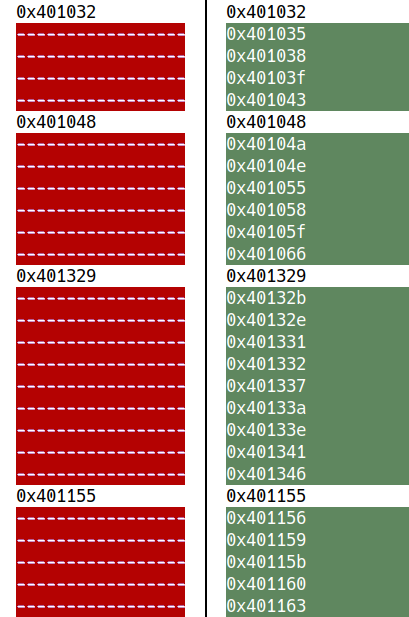
\includegraphics[width=0.6\linewidth]{figures/trace_diff_view.png}
    \caption{Different Program Trace Granularities}\label{fig:trace_granularity}
\end{figure}

This mismatch is easily resolvable: In the higher-granularity symbolic trace, merge symbolic equations for all
instructions of the same basic block into a single equation, i.e., transform the higher-granularity trace into a
lower-granularity one. This will yield larger equations, though they will not blow up exponentially as basic blocks by
definition do not include branches. A simple post-processing algorithm operating on the two traces can detect basic
block boundaries reliably because one basic block never includes the same instruction multiple times.

Problematic is the case where both granularity mismatch \textbf{and} trace divergence happen in the same trace; this is
fundamentally unsolvable in a trace post-processing scenario because one cannot differentiate between excess
instructions resulting from different branching behaviour and excess instructions from higher trace granularity.

% TODO: Move this detail to Implementation.
\subsection{Auxiliary Vector}\label{sec:auxv}

An interesting source of difference in branching behaviour between concrete- and emulator execution is the auxiliary
vector on Linux systems, which is "a mechanism that the kernel's ELF binary loader uses to pass certain information to
user space when a program is executed"~\cite{getauxval2024Mar}. Libc's initialization code (at least glibc as well as
musl libc~\cite{MuslLibc2024Feb}) iterates over that array to bring it into a representation that is indexable by entry
names, thereby depending its branching behaviour on the array's size. It turns out that QEMU, at least on some systems,
passes an auxiliary vector to the application that is different from the native auxiliary vector on the same system;
\figurename~\ref{fig:auxv_comparison} shows an example. While a customized launcher that starts both the tested emulator
and the symbolic trace recorder could in theory ensure equal environment arrays, the same is not possible for the
kernel-provided auxiliary vector.

This shows that branch-based trace mismatches are not a rare phenomenon.

\begin{figure}[htpb]
    \begin{subfigure}[t]{0.4\linewidth}
        \begin{lstlisting}
            AT_BASE : 0x790a3a4f3000
            AT_CLKTCK : 0x7ffd4e2f21b9
            AT_EGID : 0x3e8
            AT_ENTRY : 0x5d141499c050
            AT_EUID : 0x3e8
            AT_EXECFN : 0x7ffd4e2f2fec
            AT_FLAGS : 0x0
            AT_GID : 0x3e8
            AT_HWCAP : 0x64
            AT_HWCAP2 : 0x2
            AT_MINSIGSTKSZ : 0x7f0
            AT_PAGESZ : 0x1000
            AT_PHDR : 0x5d141499b040
            AT_PHENT : 0x38
            AT_PHNUM : 0xd
            AT_PLATFORM : 0xbfebfbff
            AT_RANDOM : 0x7ffd4e2f21a9
            AT_RSEQ_ALIGN : 0x20
            AT_RSEQ_FEATURE_SIZE : 0x1c
            AT_SECURE : 0x0
            AT_SYSINFO_EHDR : 0x7ffd4e349000
            AT_UID : 0x3e8
        \end{lstlisting}
    \caption{Native AUXV}
    \label{fig:native_auxv}
    \end{subfigure}
    \hfill
    \begin{subfigure}[t]{0.4\linewidth}
        \begin{lstlisting}
            AT_BASE : 0x2aaaab2ac000
            AT_CLKTCK : 0x2aaaab2ab7f9
            AT_EGID : 0x3e8
            AT_ENTRY : 0x555555557050
            AT_EUID : 0x3e8
            AT_EXECFN : 0x2aaaab2abfd1
            AT_FLAGS : 0x0
            AT_GID : 0x3e8
            AT_HWCAP : 0x64
            AT_PAGESZ : 0x1000
            AT_PHDR : 0x555555556040
            AT_PHENT : 0x38
            AT_PHNUM : 0xd
            AT_PLATFORM : 0xfcbfbfd
            AT_RANDOM : 0x2aaaab2ab7e0
            AT_SECURE : 0x0
            AT_SYSINFO_EHDR : 0x2aaaab2e3000
            AT_UID : 0x3e8
        \end{lstlisting}
        \caption{QEMU's AUXV}
        \label{fig:qemu_auxv}
    \end{subfigure}
    \caption{Comparison of auxiliary vectors in native execution and QEMU}
    \label{fig:auxv_comparison}
\end{figure}

\subsection{Experimental: A Technique for Perfectly Matching Traces}\label{sec:experimental_trace_match}

I want to outline an experimental proposal for a technique to eliminate all trace mismatches. \textbf{If} Focaccia had a
way of interfacing with a running emulator, it could read current instructions directly from the emulator's memory,
i.e., take the emulator as a source for the program trace. However, this cannot test whether the emulator decodes
instructions correctly and fails when arbitrary memory corruptions in the code area may occur; the technique is instead
useful to verify mature emulators or hand-picked selections of test cases. It can, on the other hand, give the best and
most user friendly results that Focaccia is able to compute, free of all trace-based limitations.

\section{Recording Concrete State}

The second major task, now that Focaccia can calculate truth states and compare them to emulator states, is to gather
snapshots of the tested emulator's concrete state in a representation that is usable for comparison, and do so
efficiently enough such that this part does not become a bottleneck for the entire verifier, which turned out to be
surprisingly difficult. We need one program state snapshot for each instruction that is executed.

\subsubsection{What is Program State?}

The momentary state of a program comprises the process's register- and memory content. The latter specifically being all
virtual memory pages allocated to the process in question. Everything other than these values, such as disk state,
network state, or state of peripheral hardware, is considered \textbf{input to}, not \textbf{state of} the program.

\subsubsection{Obtaining Snapshots from Emulators}\label{sec:obtaining_snapshots}

Focaccia needs a way to interface with emulators to read their state. This, of course, depends almost exclusively on
what sort of logging or debugging interfaces that are implemented by the emulator in question. The first snapshotting
mechanism that we implemented was a simple log parser specific for Arancini's log format---frankly, just because
Arancini served as the first emulator on which early prototypes of Focaccia were tested. Its log format, at that time,
was severely restricted in that Arancini exclusively wrote register values to the log, but no memory content. The latter
is always a challenge for static, non-interactive communication paths like log files as their size can easily blow out
of proportion for even moderately sized programs when the emulator dumps \textit{all} memory to disk at every
instruction. Additionally, almost all memory is never touched by each given instruction (a typical non-vector
instruction addresses 16 bytes of memory at most) and is thus not strictly required by the verifier.

The fact is that Focaccia will always have to deal with incomplete snapshots and missing information from input data.
Whether this is because of faults in the emulator, restricted communication interfaces, or incomplete format conversion
implementations: the reason is outside of our control and one cannot create information, therefore, we always have to
deal with its abscence. From this insight, we derived a key architectural principle for the verifier: It must not assume
the presence of any information, fail gracefully if key information is indeed missing, and, most importantly, scale the
quality of its calculations incrementally with more information.

But back to the matter at hand: Log files are a well decoupled solution that only requires a single parsing function to
be implemented to support a new emulator. On the other hand, dumping memory to files in a large-scale fashion is very
costly and the emulator has to \textbf{support} dumping memory to logs in the first place. Our major evaluation target,
QEMU, does not. Another more memory-efficient approach is an online debugging interface, such as the one QEMU provides
by implementing the \texttt{gdbserver} protocol. This method is less intrusive to Focaccia (in fact, it demands no
modification of Focaccia at all to interface with new emulators) but moves some of the effort to the side of the
emulator, at which the responsibility lies to implement said protocol.

\subsubsection{Recording QEMU State}

QEMU has extensive options for logging output, but it cannot write memory to the log. Additionally, even though logging
can output memory mapping informations, QEMU's \texttt{gdbserver}-based remote debugging interface can not, so that
there is no obvious way to know which memory addresses exactly to include in the snapshot. The result was a rather
inventive first iteration of a customized snapshotting system for QEMU, for which
\figurename~\ref{fig:qemu_naive_recording} gives a high-level visualization.

\begin{figure}[htpb]
    \centering
    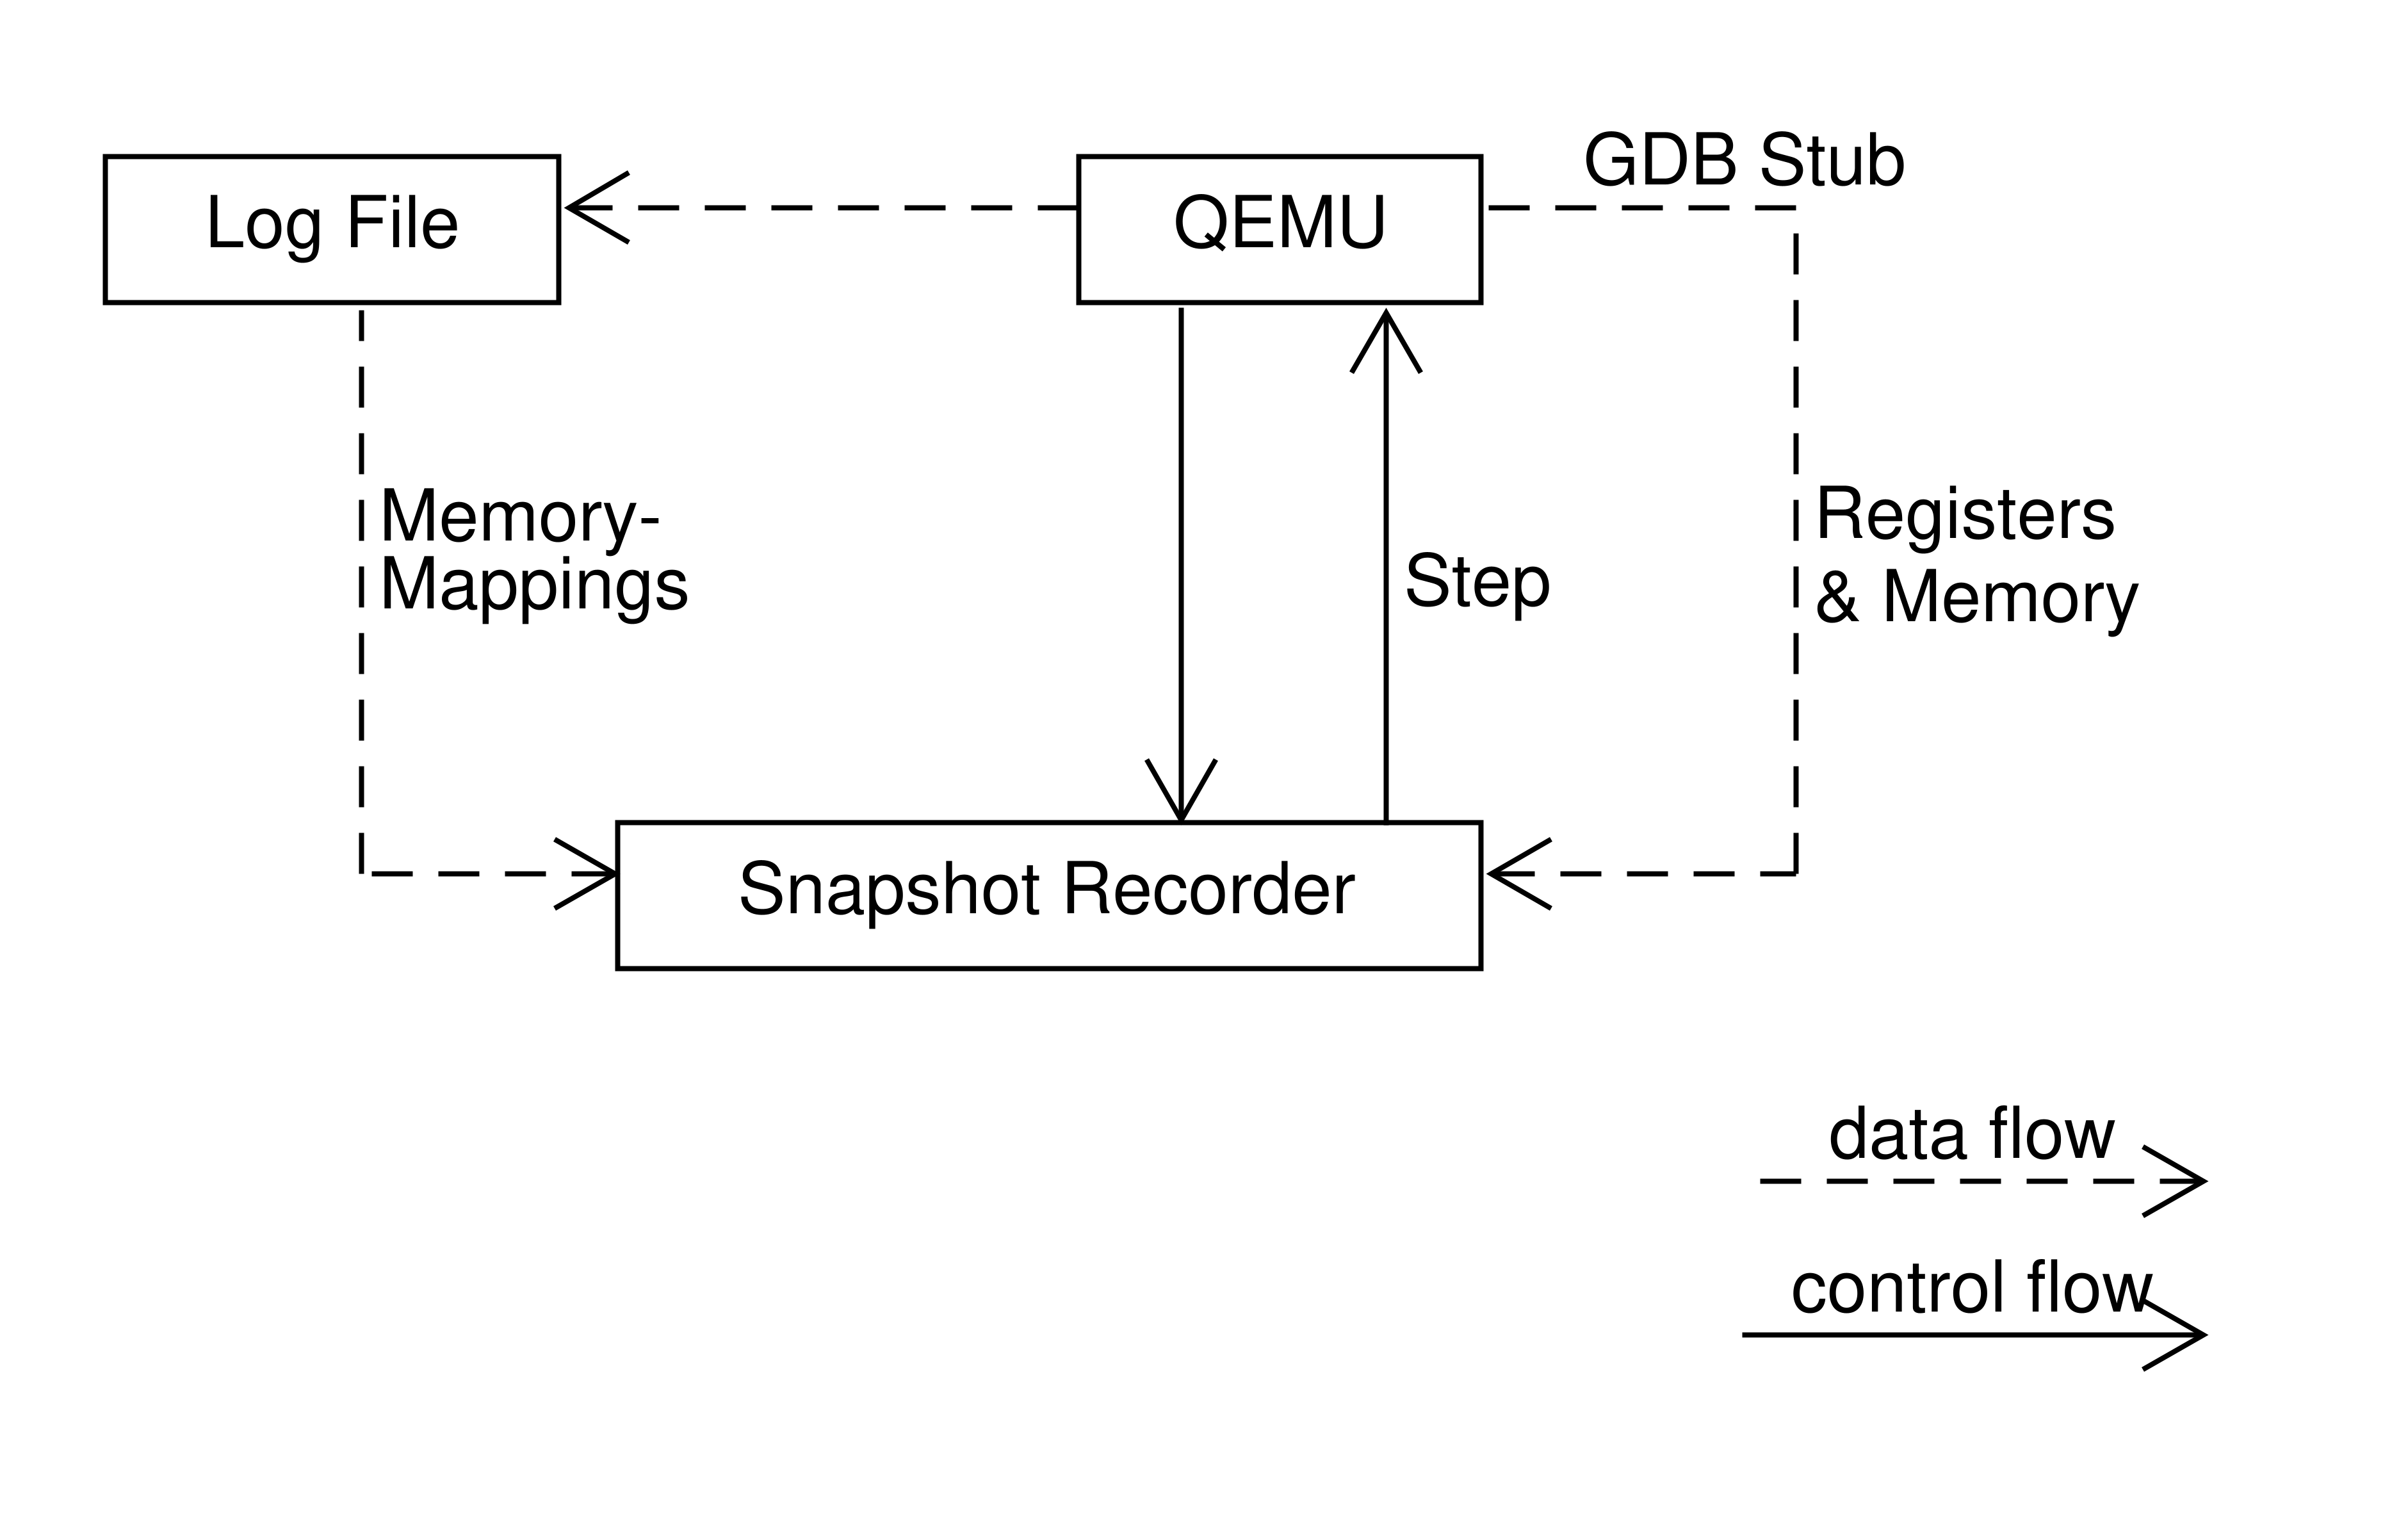
\includegraphics[width=0.8\linewidth]{figures/qemu_naive_recording.png}
    \caption{Recording QEMU Snapshots}\label{fig:qemu_naive_recording}
\end{figure}

The snapshot recorder is an algorithm that does multiple things. First, it starts an instance of QEMU, passing to it
several options that enable logging and the \texttt{gdbserver} stub, which makes QEMU wait before the first instruction
until a connected GDB instance instructs it to start execution. The script then connects to the GDB stub, which it uses
from there on to read register- and memory values from QEMU, and also to step its execution forward by increments of
single instructions. To know what bytes of memory to record, it simultaneously reads from QEMU's log file, to where QEMU
outputs its memory mappings every time they change (e.g., when a new page is allocated). The recorder thus keeps track
of the memory pages allocated to the emulated process and records at each instruction all content of all allocated
pages, in addition to all register contents, in a snapshot.

Unfortunately, this approach turned out not only to be highly memory inefficient seeing as almost all memory of a
process is irrelevant for each given single instruction, but also exceedingly slow---so much so that the system was
virtually unusable: For a minimal `Hello World`-program, which, compiled with \texttt{musl libc}, results in a trace of
1106 instructions on our test system and compiler version, the memory footprint of an average snapshot is around 2.2
megabytes and the average time taken to read that amount of data over QEMU's GDB stub is around $185$ milliseconds,
resulting in a total 15.88 gigabytes of snapshot data recorded over 321 seconds, or 5.35 minutes, of execution time.

These results are unacceptable to any productive development setting, not to mention that the solution is entirely
specific to QEMU and cannot be transferred to other emulators easily. The evolution of this system is our
\textit{minimal snapshotting} approach. It reduces the amount of data stored in each snapshot to the theoretical minimum
that is required for the verifier to compute its results, while simultaneously removing the reliance on a specific log
structure by moving to a purely \texttt{gdbserver}-protocol-based interface. Even this interface is highly exchangeable
with any remote communication protocol as long as it supports three basic commands: Reading memory content at arbitrary
addresses, reading register content, and stepping the program forward by single instructions. The following section
explains all of this in detail.

\subsubsection{Minimal snapshots}\label{sec:minimal_snapshots}

A key capability that interactive remote debugging interfaces to running emulators enable for the snapshotting engine is
that it can \textbf{choose} which parts of the emulator's state it wants to record (in contrast, for example, to static
log files where the emulator chooses which data to dump). By considering as additional information the symbolic
representation of an instruction's semantics, it can calculate the exact subset of a program's state that is needed to
verify only that instruction, and record it in a \textit{minimal snapshot}.

Minimal data to verify the correctness of one instruction encompasses information from \textbf{two} program states: The
input state to the instruction, i.e., the state on which the instruction acts, and its output state, i.e., the state
that the instruction produces; the former to compute the expected reference destination state, the latter to compare it
to the reference state. Relevant data of the input state are input values to the instruction (its \textit{source
operands}), while that of the output state encompasses the instruction's output values (its \textit{destination
operands}). We can determine both from an instruction's symbolic equations.

\tikzstyle{state_node} = [rectangle, draw=black, text centered, minimum width=2cm, minimum height=1cm]
\tikzstyle{arrow} = [thick, ->, >=stealth]

%\begin{wrapfigure}{R}{0.3\textwidth}
\begin{figure}[htpb]
\begin{center}
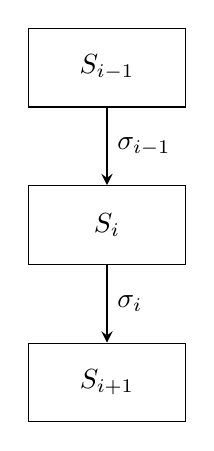
\begin{tikzpicture}[scale=1, transform shape, node distance=2cm]
    \node (prev) [state_node] {$S_{i-1}$};
    \node (cur)  [state_node, below of=prev] {$S_{i}$};
    \node (next) [state_node, below of=cur] {$S_{i+1}$};

    \draw [arrow] (prev) -- node[anchor=west] {$\sigma_{i-1}$} (cur);
    \draw [arrow] (cur)  -- node[anchor=west] {$\sigma_{i}$} (next);
\end{tikzpicture}
\end{center}
\caption{Instruction data flow}%
\label{fig:instr_data_flow}
\end{figure}
%\end{wrapfigure}

To create a minimal snapshot $s_i$ from a full program state $S^E_i$ so that it has all data required by the verifier to
calculate the comparison to its respective truth state $\Delta_{S_i} = S_i - S^E_i$ and also calculate the next expected
truth state $S_{i+1} = \sigma_i(S^E_i) = \sigma_i(s_i)$ from it, the following information is required:

\begin{itemize}
    \item $\sigma_{i-1}$: A representation of the transformation that produces $S_i$. Determines the destination
        operands of $x_{i-1}$, the values of which are required to compare $S^E_i$ to the expected truth state.
    \item $\sigma_i$: A representation of the transformation that acts on $S^E_i$. Determines the source operands of
        $x_i$, the values of which are used to calculate the next truth state $S_{i+1}$ that will be compared to
        $S^E_{i+1}$.
    \item $S^E_{i-1}$: The previous program state on which producing instruction $x_{i-1}$ acts. We need it to record
        $s_i$ because symbolic addresses of memory accesses in $x_{i-1}$'s destination operands, which must be included
        in $s_i$, depend on it. Example: for $x_{i-1} = \texttt{mov [rsp],rax}$, we need to know the value of
        \texttt{rsp} in $S^E_{i-1}$ so that we can include memory at that address in $s_i$.
    \item $S^E_i$: The current emulator state that is to be reduced to $s_i$.
\end{itemize}

\paragraph{Example} The instruction $x = \texttt{ADD [RDI+0x20], RAX}$ calculates \texttt{RAX + 64@[RDI+0x20]} and
stores the result in \texttt{[RDI+0x20]}, also modifying some state flags in the process. We shall call the emulated
program state before the instruction is executed $S^E_0$ and the emulated state after the instruction $S^E_1 =
E(x)(S^E_0)$.

The snapshot of the state $S^E_0$ must contain at least the register \texttt{RAX} and 8 bytes of memory
\texttt{64@[RDI+0x20]} so that the expected state $S_1 = x(S^E_0)$ can be calculated. The snapshot of the emulator state
$S^E_1$ must contain the output values \texttt{64@[RDI+0x20]} and \texttt{RFLAGS} so that the comparison $S_1 = S^E_1$
can be performed. Additionally, because the memory address to which the instruction writes is based on \texttt{RDI}'s
value in $S_0$, not in $S_1$, the snapshot of $S_0$ must also store \texttt{RDI} so that the following state can
calculate the address \texttt{[RDI + 0x20]}. In the context of a continuous trace, the second snapshot must also contain
all inputs to the next instruction, and so forth.
\\

When we apply this technique to record snapshots from QEMU in the same testing environment as used in the measurings
above, the algorithm generates a total of 121 kilobytes of snapshot data (a large part of which is overhead from the
admittedly far from optimized JSON format we use to serialize snapshots) recorded over a total of 6.9 seconds. This is a
reduction in space consumption of 13,123,900\% and a 4,650\% reduction in execution time.

% Problems with this approach
However, minimal snapshots, as always, introduce a new restriction: The algorithm can now establish only a \textit{lower
bound} on emulator correctness, that is, tell whether an instruction does \textbf{at least} what it is supposed to do.
With entire-memory snapshots, an upper bound, which means that an instruction does \textbf{at most} what it is supposed
to do, would have been possible to establish because its calculation does not inherently suffer from the $\Delta_S$
problem---the only thing that needs to be tested is whether all values that should \textbf{not} have been touched by an
instruction have remained the same, no matter their concrete value. Obviously, establishing both an upper- and a lower
bound would imply certainty that an instruction does \textbf{exactly} what it is supposed to do. With minimal snapshots
and all of the benefits that go along with them, however, that becomes impossible since the data required for the
calculation is not present anymore.



% APPROACH
%
%  - systematic!
%  - we don't want to write tests
%  - fuzzing has more setup work, is harder to use
%
% chapter 12 virtual machines popek & goldberg
%
% establishing V(S_j)
